% Chapter Template

\chapter{Software Framework} % Main chapter title

\label{Chapter4} % Change X to a consecutive number; for referencing this chapter elsewhere, use \ref{ChapterX}

\lhead{Chapter 4. \emph{Software Framework}} 
The ROS \cite{quigley2009ros} is the de facto standard used for any robotics related research in the recent times. However it is officially supported only for the Ubuntu distribution which makes it unavailable to the people who work with sensors that are being supported say only for Microsoft Windows Platform (i.e Kinect for Windows v2). Hence a distributed architecture which is not specific to any operating system or programming language is proposed which uses open network communication standards and transparent message passing using structured data. In this chapter the design philosophy of the software framework and core components of the system are explained.
		
\section{Framework Design}		
	The system contains nodes/processes which can be running in the same computer or might be running anywhere in the network. The order of start and stop of these nodes essentially do not matter.
\subsection{Communication Protocol}	
	The nodes communicate with each other as shown in Fig~\ref{fig:framework} using either of inproc/IPC/TCP/UDP protocols depending on its location and to whom it wants to communicate with. The communication between the nodes is established using ZeroMQ \cite{ZeroMQ} library which has a variety of advantages any modern application would require like  
\begin{itemize}
\item Multiple language and cross platform
\item Message using inproc, IPC, TCP, UDP protocols
\item Support for patterns like Publisher-Subscriber, Push-Pull, Request-Response
\item Tiny and high-speed asynchronous implementation
\end{itemize}
	ZeroMQ comes with the low-level C API. High-level bindings exist in 40+ languages including Python, Java, PHP, Ruby, C, C++, C\#, Erlang, Perl, and more. So it can run in literally any OS and owing to its very low memory foot print it can also run on the mobile devices and tablets.
\begin{figure}
\centering
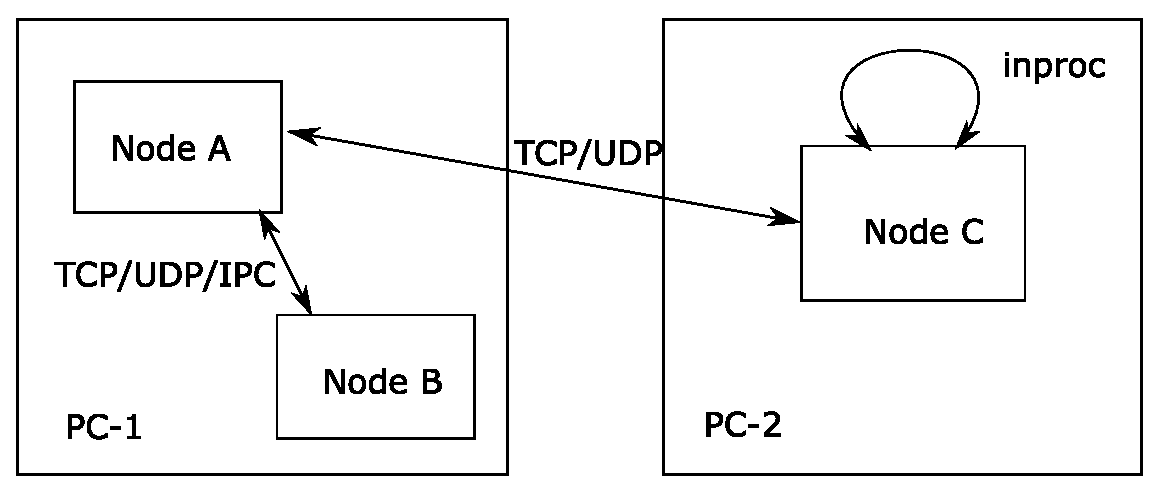
\includegraphics[width=\textwidth]{assets/architecture_comm.eps}
\caption[Framework Communication Protocol]{Framework Communication Protocol}
\label{fig:framework}
\end{figure}
\subsection{Message Format}
	The nodes communicate with each other using structured data formatted using the Google Protocol buffers \cite{ProtocolBuffers}. Protocol buffers are Google's language-neutral, platform-neutral, extensible mechanism for serializing structured data. It could be thought of as XML format, but smaller, faster, and simpler. The data could be structured once as per the requirement, then the special generated source code could be integrated with the application to easily write and read structured data to and from a variety of data streams and using a variety of languages – Java, C++, C\# or Python. The message is defined in a file with extension *.proto which will be consumed by the code generator to generate code for a specific language. A sample proto file is shown in Fig~\ref{fig:protobuf_def} and the code generation principle is shown in Fig~\ref{fig:protobuf_codegen}
\begin{figure}
\centering
\begin{subfigure}[t]{0.48\textwidth}
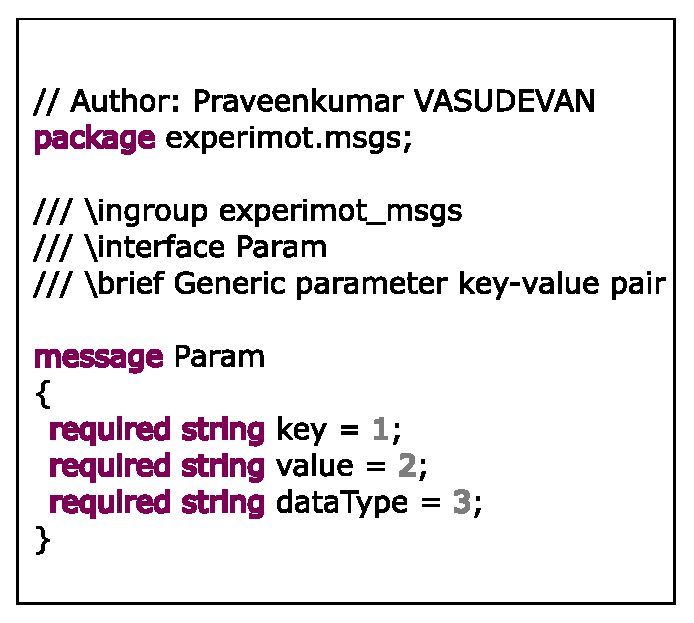
\includegraphics[width=\textwidth]{assets/protobuf_definition.eps}
\caption[Message Definition]{Message Definition}
\label{fig:protobuf_def}
\end{subfigure}
\begin{subfigure}[t]{0.48\textwidth}
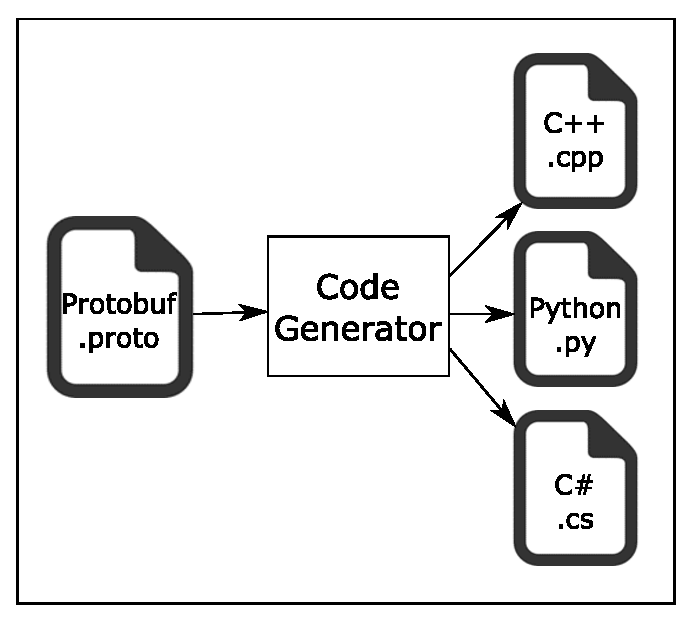
\includegraphics[width=\textwidth]{assets/protobuf_codegen.eps}
\caption[Code Generation]{Code Generation}
\label{fig:protobuf_codegen}
\end{subfigure}
\caption[Google Protocol Buffers]{Google Protocol Buffers}
\label{fig:protobuf}
\end{figure}
\subsection{Configuration File}
\label{sec:config_file}
	An XML configuration file to manage the nodes and system/node level parameters is proposed. The format of the XML file is designed using XML schema definition (XSD) language. The schema representation is shown in the Fig~\ref{fig:config_xsd}. The important strongly typed components of the schema are
	\begin{itemize}
	\item Parameters: These are the global parameters composed of key, value and type of the parameter. The supported types are boolean, integer, double, string and comma separated values(CSV). 
	\item Nodes: These are the individual processes that would compose the application as a whole. Each of these nodes could be written in any programming language supported by the communication protocol and message serialization library. Each node in turn is composed of
	\begin{itemize}
	\item Name : A name unique to this node
	\item Enable/Disable Flag: A flag to tell the application if this node has to be started when the application starts up.
	\item Type: The type is the user-defined role of the node.
	\item Process Information: The executable/script along with a set of arguments associated with this node.
	\item Parameters: These are the node level parameters with the structure similar to the global parameters. A node level parameter can override the global parameter with the same name.
	\item Publishers: A set of publisher which publishes a message (structured using proto format) on a specific topic over a configured communication channel (TCP/UDP/IPC etc.,). Usually the publishers relates to the data produced by this node.
	\item Subscribers: A set of subscriber which listens to a message of specific type published on a specific topic over a specific communication channel. The subscribers relates to the data consumed by this node.
	\end{itemize}
	\end{itemize}
\begin{figure}
\centering
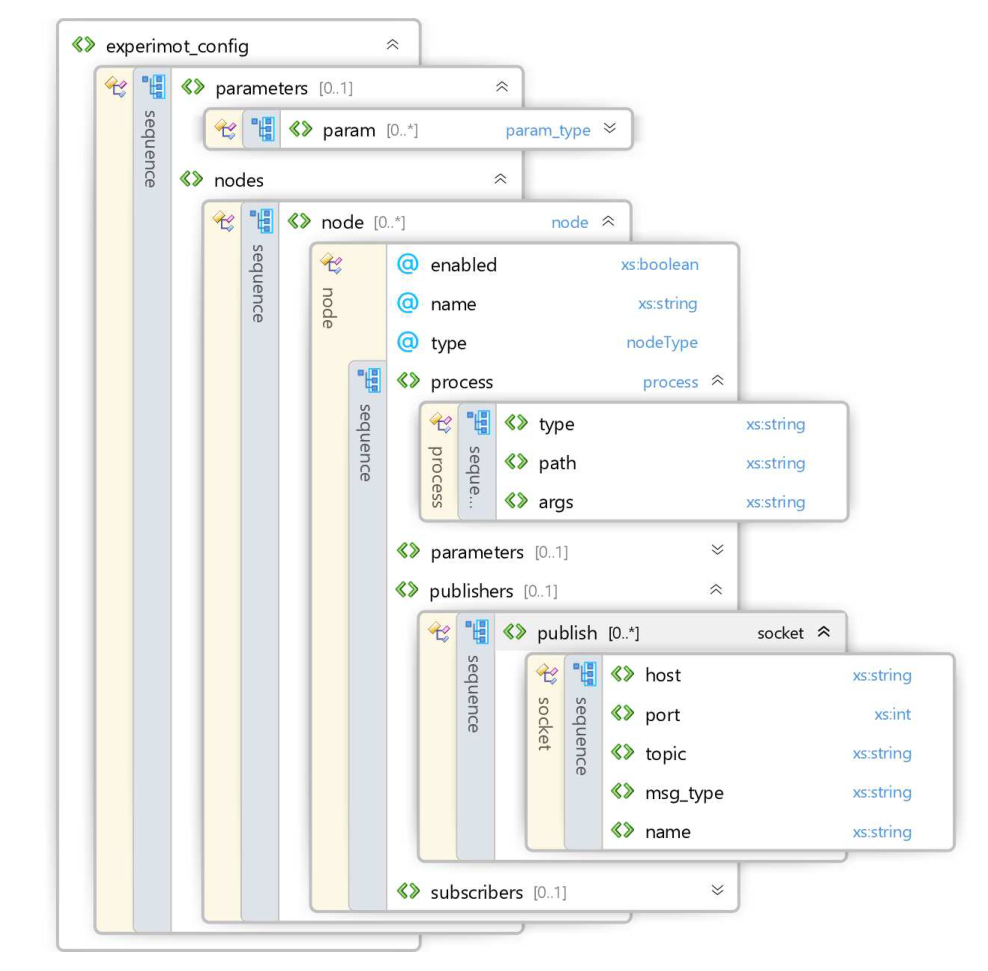
\includegraphics[width=\textwidth]{assets/xsd_config.eps}
\caption[Configuration XML Schema Definition]{Configuration XML Schema Definition}
\label{fig:config_xsd}
\end{figure}
\subsection{An example usage of the framework}
In order to demonstrate how the framework described so far could be used for developing a distributed application, a sample application scenario is considered. A \emph{robot\_interace\_node} node reads the joint values of the robot and publishes them over a topic \textbf{RJV} (robot joint values). Another node namely \emph{visualization\_node} subscribes to the topic \textbf{RJV} and each time it receives the new joint values updates the joint position of the robot being shown by the visualization engine. The pseudo-code of these nodes are shown in Fig~\ref{fig:node_a} and Fig~\ref{fig:node_b} respectively.
\begin{figure}[H]
%\centering
\begin{subfigure}[t]{0.48\textwidth}
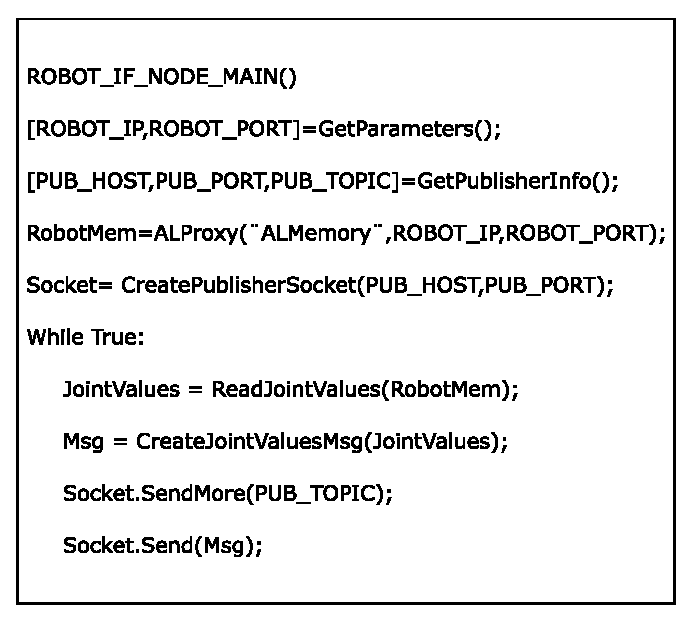
\includegraphics[width=\textwidth]{assets/sample_node_A.eps}
\caption[Robot Interface Node]{Robot Interface Node}
\label{fig:node_a}
\end{subfigure}
\begin{subfigure}[t]{0.48\textwidth}
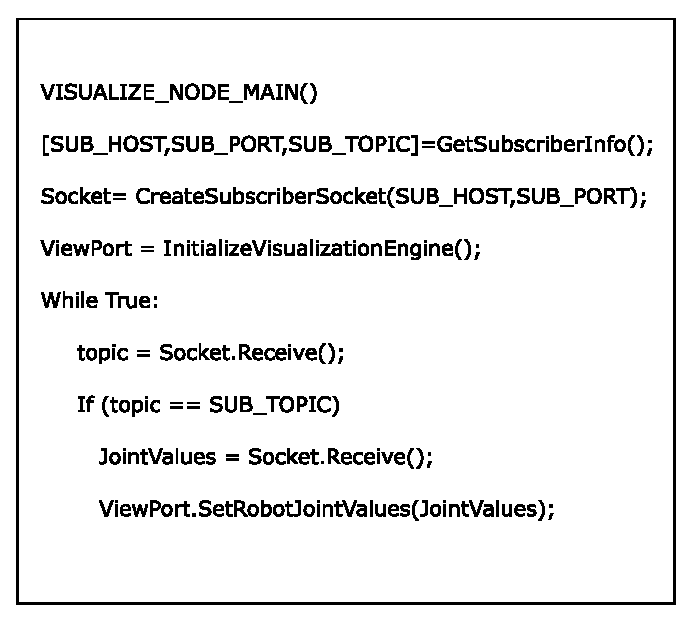
\includegraphics[width=\textwidth]{assets/sample_node_B.eps}
\caption[Visualization Node]{Visualization Node}
\label{fig:node_b}
\end{subfigure}
\caption[Sample nodes]{Sample nodes}
\label{fig:pseudo_nodes}
\end{figure}
And finally we can define a configuration file which contains the parameters and start up information needed by the application to start up these nodes. A sample configuration file for this scenario is shown in Listing~\ref{lst:sample_config}

\lstinputlisting[caption=Sample XML Configuration File,label={lst:sample_config},language=XML]{assets/sample_config.xml}

\section{User Interface Design}
\label{sec:ui_design}
The applications targeted for naive users should be designed carefully in order to abstract the complex architecture details and reduce the number of steps the user has to follow in order to do what he/she desires. Hence obviously terminal based command interfaces are not suitable since they may be daunting even for intermediate programmers. A simple and intuitive user interface is inevitable under such scenarios where visual programming techniques come into the picture. Additionally the application hosting the user interface could be a native application targeted to any particular operating system say Windows, Linux, OSX, iOS, Android etc., This will once again restrict the usage requiring the user to have that particular OS installed in their device. The web applications come handy which could tackle all the aforesaid bottlenecks. Hence for the experimental platform, an user interface which is based on latest web standards (HTML5, CSS3, WebGL etc.,) is proposed. It is perfectly suited for smart environments which adopts ``Bring your own device'' policy. In this section the libraries that have been used for building up the user interface is explained.

\subsection{Web Frameworks}
	The web application development has been reaching newer heights in recent times. The web revolution has led to the development of wide variety of libraries and frameworks in order to make the application creation way simpler than ever before. The user interface has been strengthed by a number of libraries and a summary of the libraries used is described below.

\begin{itemize}
\item \emph{Three.js}: Three.js is a JavaScript 3D library that offers a wide range of features for creating and displaying 3D computer graphics on a web browser in an intuitive manner using JavaScript without having to deal with the complexity of a WebGL low-level API. It is also suitable for mobile and desktop environment. This makes it ideal for hosting virtual 3D environments and dispaly simulation of human robot interaction.
\item \emph{jQuery}: jQuery is a fast, small, and feature-rich JavaScript library. It makes things like HTML document traversal and manipulation, event handling, animation, and Ajax much simpler with an easy-to-use API that works across a multitude of browsers. With a combination of versatility and extensibility, jQuery has changed the way that millions of people write JavaScript.
\item \emph{jQuery-UI}: jQuery UI is a curated set of user interface interactions, effects, widgets, and themes built on top of the jQuery JavaScript Library. Whether you're building highly interactive web applications or you just need to add a date picker to a form control, jQuery UI is the perfect choice.
\item \emph{Backbone.js}: Backbone.js gives structure to web applications by providing models with key-value binding and custom events, collections with a rich API of enumerable functions, views with declarative event handling, and connects it all to your existing API over a RESTful JSON interface.
\item \emph{Underscore}: Underscore is a JavaScript library that provides a whole mess of useful functional programming helpers without extending any built-in objects. Underscore provides helper functions like map, filter, invoke as well as more specialized goodies like function binding, javascript templating, creating quick indexes, and so on.
\item \emph{Marionette}: Marionette simplifies your Backbone application code with robust views and architecture solutions. It helps organize the application in terms of small views and makes it easy to compose rich layouts out of small components. It also provides decoupled communication between application components with a powerful messaging system.
\end{itemize}

\subsection{Blockly: Visual Programming Editor}
Blockly \cite{Blockly} is a library for building visual programming editors. It allows users to write programs by plugging blocks together. Developers can integrate the blockly editor into their own web applications to create a great UI for novice users. It is being used by hundreds of projects as a visual editor. The main features of the Blockly library are as follows

\begin{itemize}
\item Compact, Open source and Web-based, no Flash.
\item Supports a wide range of web browsers: Google Chrome, Firefox, Safari, Opera, IE.
\item Android and iOS support.
\item Support for Variables, functions, arrays etc.,
\item Syntax errors are impossible.
\item Basic type checking.
\item Extendible with custom blocks.
\item Code generation API available for Javascript, Python, and more.
\item Suitable for touch based interface.
\end{itemize}

\begin{figure}[H]
%\centering
\begin{subfigure}[h]{0.48\textwidth}
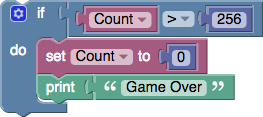
\includegraphics[width=\textwidth]{assets/blockly_sample.png}
\caption[Visual Program]{Visual Program}
\label{fig:blockly_sample}
\end{subfigure}
\hfill
\begin{subfigure}[h]{0.48\textwidth}
\lstinputlisting[language=Python]{assets/blockly_sample.txt}
\caption[Generated code]{Generated code}
\label{fig:blockly_sample_code}
\end{subfigure}
\caption[Google Blockly editor]{Google Blockly editor}
\label{fig:pseudo_nodes}
\end{figure}

Fig~\ref{fig:blockly_sample} shows a simple program that could be created with blockly. Then Blockly provides API to generate the corresponding code in JavaScript, Python, PHP, Dart, or some other language. For instance the Python code corresponding to the sample visual program is shown in Fig~\ref{fig:blockly_sample_code}

The application can then execute the code as desired. From the application developer's point of view, Blockly is basically a textarea into which the user types syntactically perfect code.  Blockly makes it completely impossible to make a syntax error. There are no unbalanced parentheses, no unescaped strings, no missing semicolons. Blockly allows novice programmers to concentrate on the logic.

Additionally, many non-programmers find a blank screen with a blinking cursor to be daunting. Even seasoned programmers can benefit by starting a script with Blockly. Blockly makes it easy to create custom blocks and code generation which simplifies the task of developers to create application specific programming language interface for novice users. All these advantages makes Blockly ideal fit for creating robot behavior programs by novice programmers.

\section{Summary}

This chapter explained the software design philosophy behind the experimental platform. The software makes use of open communication standards, messaging sytems and web application standards. This systematic approach ensures the integrity and robustness to the rapidly changing software technologies. The framework also benefits from a lot of community driven open source projects which makes sure that the code is robust and has undergone tests in different use cases. The list of all tools, technologies and libraries used to build the experimental platform is shown in Fig~\ref{fig:libraries_used}
\begin{figure}
\centering
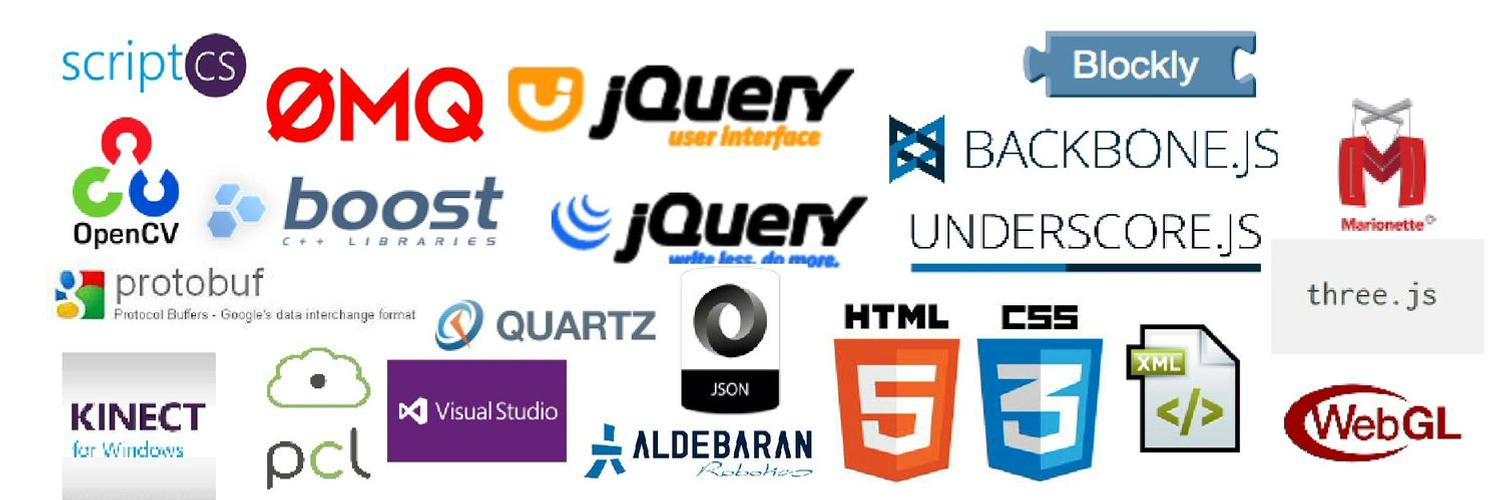
\includegraphics[width=\textwidth]{assets/libs.jpg}
\caption[Technologies, Tools \& Libraries]{Technologies, Tools \& Libraries}
\label{fig:libraries_used}
\end{figure}
